\documentclass[14pt]{extarticle}
\usepackage{fontspec}
\usepackage{indentfirst}
\linespread{1.5}
\usepackage{polyglossia}
\usepackage{enumitem}
\setdefaultlanguage{russian}
\usepackage[table]{xcolor}
\usepackage[listings]{tcolorbox}
\usepackage{makecell}
\usepackage{graphicx}
\usepackage{nameref}
\usepackage[tiny]{titlesec}
\usepackage{amsmath}
\usepackage{amssymb}
\usepackage{caption}
\usepackage{hyperref}
\usepackage{wrapfig}
\usepackage{multirow}
\setcounter{page}{4}
\usepackage{tabularx}

\newcommand{\cy}{\cellcolor{yellow!25}}
\newcommand{\cg}{\cellcolor{green!25}}
\newcolumntype{P}{>{\raggedleft\arraybackslash}p{.2in}}
\definecolor{std-color}{rgb}{0.144531, 0.554688, 0.554688}
\definecolor{type-color}{rgb}{0.0, 0.0, 0.699219}
\definecolor{string-color}{rgb}{0.3333, 0.5254, 0.345}
\definecolor{key-color}{rgb}{0.8, 0.47, 0.196}
\definecolor{cmnt-color}{rgb}{0.5, 0.5, 0.5}

\lstset { %
	language=C++,
	numbers=left, 
	numberstyle=\small\color{gray},
	frame=top,
	frame=bottom,
	upquote=true,
	stepnumber=1,
	numbersep=8pt,
	showstringspaces=false,
	basicstyle =\small\ttfamily,
%	backgroundcolor=\color{black!5}, % set backgroundcolor
%	basicstyle=\ttfamily,% basic font setting
%	basicstyle=\ttfamily,
	keywordstyle=\color{blue},
	 keepspaces=true,
%	stringstyle=\color{red}\ttfamily,
%	commentstyle=\color{green}\ttfamily,
%	morecomment=[l][\color{magenta}]{\#}
	xleftmargin=-1cm, xrightmargin=1.3cm,
	escapeinside={<@}{@>}
}

\lstdefinestyle{mystyle}
{
	language = C++,
	inputencoding=utf8x, 
	extendedchars=\true,
	basicstyle = {\ttfamily \color{black}},
	%backgroundcolor = {\color{back-color}},
	stringstyle = {\color{string-color}},
%	commentstyle=\color{green}\ttfamily,
	keywordstyle = {\color{blue}},
	keywordstyle = [2]{\color{std-color}},
	keywordstyle = [3]{\color{type-color}},
	keywordstyle = [4]{\color{cmnt-color}},
	morekeywords = [2]{std, vector, clbool, coo, Controls, matrix\_coo},
	morekeywords = [3]{uint32\_t, uint},
%	morekeywords = [4]{//, данные, для, матри.цы, A}
}



\newcommand{\sectionbreak}{\clearpage}
\newcommand{\txt}{\textit}
\newcommand{\bld}{\textbf}

\titleformat{\section}
{\normalfont\fontsize{16}{15}\bfseries}{\thesection}{1em}{}

\titlespacing\section{0pt}{12pt plus 4pt minus 2pt}{0pt plus 2pt minus 2pt}
\titlespacing\subsection{0pt}{12pt plus 4pt minus 2pt}{0pt plus 2pt minus 2pt}
\titlespacing\subsubsection{0pt}{12pt plus 4pt minus 2pt}{0pt plus 2pt minus 2pt}

\setdefaultlanguage{russian}
\setmainfont{Times New Roman}
\setsansfont{Times New Roman}
\setmonofont{Arial}


\usepackage{fancyhdr}

\usepackage{geometry}
\geometry{
	a4paper,
	left=30mm,
	top=20mm,
	bottom=20mm,
	right=15mm,
	headsep=0pt
}

\fancyhf{}


\addto\captionsrussian{% Replace "english" with the language you use
	\renewcommand{\contentsname}%
	{Оглавление}%
}


\setlength{\parindent}{1.25cm}

\begin{document}\sloppy

\tableofcontents
	 
\section*{Введение}
\label{sec:intro}
\addcontentsline{toc}{section}{Введение}
	 Во множестве областей данные естественно представлять в виде графов -- веб и интернет, биоинформатика, социальные сети, дорожные карты. Анализ и обработка таких данных включает в себя работу с графами. Постоянный рост количества данных задает серьезные требования к производительности алгоритмов анализа графов. 
	 
	 Многие операции с графами эквивалентны операциям с их матрицами смежности, что позволяет выразить их в терминах линейной алгебры. Например, поиск кратчайших путей и транзитивное замыкание описываются возведением матрицы в степень. Сведение алгоритмов к операциям линейной алгебры над некоторым полукольцом позволяет использовать возможности массового параллелизма GPGPU.
	 
	 Базовые операции линейной алгебры, такие как сложение и умножение матриц, можно использовать в качестве компонент сложных алгоритмов анализа графов. Необходимость научного сообщества в таких операциях способствовала появлению стандарта GraphBLAS\cite{graphblas}, описывающего интерфейсы операций линейной алгебры, которые наиболее часто встречаются в алгоритмах на графах. Создатели GraphBLAS вдохновлялись появившимся ещё в 70-х годах стандартом базовых подпрограмм линейной алгебры BLAS. Различие стандартов в первую очередь заключается в наборе базовых операций. Оба стандарта содержат умножение матриц, но произведение Кронекера есть только в GraphBLAS, так как оно часто встречается в графовых алгоритмах.
	 
	 Матрицы смежности многих реальных графов оказываются сильно разреженными, то есть в основном состоят из нулевых элементов. Для хранения и обработки разреженных матриц используют сжатые форматы. Эффективно реализовать некоторые операции с разреженными матрицами на GPU достаточно сложно, особенно это касается умножения матрицы на вектор и матрицы на матрицу. 
	 
	 На текущий момент можно найти только одну полную реализацию стандарта GraphBLAS с поддержкой булева полукольца на CPU в библиотеке SuiteSparse \cite{suite_sparse}. Активные разработки GraphBLAS API с использованием GPGPU сейчас ориентированы на CUDA, что ограничивает весь набор высокопроизводительных устройств видеокартами от NVIDIA. Ориентация на OpenCL позволит исследователям использовать и другие устройства -- карты AMD, матрицы FPGA, а также запускать имеющийся код на CPU.  
	  
	 \sectionbreak
	 
\section*{Цель и задачи}
\label{sec:goals}
\addcontentsline{toc}{section}{Цель и задачи}

	 Данная работа была мотивирована появлением матричных алгоритмов для контекстно-свободных запросов к графам -- CFPQ. На данный момент CFPQ не поддерживаются большинством графовых баз данных, так как современные решения всё ещё не обладают достаточной производительностью \cite{kup}. В лаборатории языковых инструментов JetBrains исследуется производительность матричных алгоритмов CFPQ \cite{cfpq_all} с целью достижения их практической применимости.
	 
	 Все матричные операции исследуемых алгоритмов осуществляются над матрицами смежности разреженных графов. Элементы матрицы смежности принимают значения 0 или 1, то есть такие матрицы являются булевыми.
	 
	 В рамках исследований необходимые операции ранее были реализованы на CUDA. Мы будем опираться те же идеи и алгоритмы, но попробуем и другие матричные форматы с целью экономии памяти в случае сверхразреженных матриц.
	 
	 \textbf{Целью} работы является реализация OpenCL библиотеки с операциями для разреженных булевых матриц, необходимыми для реализации матричных алгоритмов CFPQ.
	 
	 \textbf{Задачи}:
	 \begin{enumerate}[itemsep=0mm, topsep=0pt]
	 	\item Реализация следующих операций над разреженными булевыми матрицами:
	 	\begin{enumerate}[itemsep=0mm, topsep=0pt]
	 		\item[--] матричное умножение,
	 		\item[--] матричное сложение,
	 		\item[--] транспонирование матрицы,
	 		\item[--] извлечение подматрицы,
	 		\item[--] редуцирование строк матрицы,
	 		\item[--] произведение Кронекера.
	 	\end{enumerate}
	 	\item Оформление результатов в библиотеку операций с разреженными булевыми матрицами.
	 	\item Экспериментальное исследование библиотеки: 
	 	\begin{enumerate}[itemsep=0mm, topsep=0pt]
	 		\item[--] сравнение производительности отдельных операций с существующими решениями на видеокарте NVIDIA,
	 		\item[--] сравнение производительности отдельных операций на различных устройствах: NVIDIA, AMD, FPGA.
	 	\end{enumerate}
	 	
	\end{enumerate}
	 
	 
	 Мы рассчитываем, что наши реализации матричных операций позволят улучшить производительность алгоритмов анализа графов, выраженных в терминах линейной алгебры. 
	 
	 \sectionbreak
	 
\section{Обзор предметной области}	

	\subsection{Вычисления GPGPU}
	
	Видеокарты были изобретены для задач компьютерной графики. Сотни и тысячи маленьких вычислительных юнитов идеально подошли для параллельной обработки несложных задач: вычисление цветов треугольников, их позиций, нормалей, текстур и попиксельной обработки. 
	
	Со временем модель массового параллелизма начали использовать для неграфических задач, и так появилась техника GPGPU -- General-purpose computing on graphics processing units. GPGPU активно используется в физике, машинном обучении, математике. Многие классические алгоритмы перенесены на архитектуру видеокарт: префиксная сумма, различные сортировки, свертки массивов, слияние массивов.
	
	В графике видеокарта исполняет код шейдеров -- программ на языке glsl, а в GPGPU они были заменены ядрами на языках C и С++. Возможность создавать и исполнять программы GPGPU поддерживают два основных фреймворка -- CUDA и OpenCL. 
	
	Операции с плотными матрицами хорошо ложатся на модель GPGPU. Они удобно делятся на простые и равные по вычислительной сложности подзадачи и позволяют достичь существенного прироста в скорости. Для операций с разреженными матрицами выделить подзадачи становится сложнее.
	
	
	
	Создавая решения для видеокарты, необходимо учитывать ряд её архитектурных особенностей, иначе в результате можно не достигнуть поставленных целей. На рисунке \ref{fig:smnvidia} представлена архитектура одного SM\footnote{Streaming multiprocessor -- планировщик работы вычислительных юнитов видеокарты}, из которых состоит видеокарта. За работу одного потока отвечает простое вычислительное устройство -- Core или ALU. 32 таких устройства образуют \emph{ворп}. Потоки ворпа обладают одним указателем на инструкции и в пределах одного мультипроцессора могут взаимодействовать друг с другом через \emph{локальную память}, механизм блокировок и CAS-операции. Всем вычислительным устройствам доступна \emph{глобальная память}, через которую потоки получают данные и куда записывают результаты вычислений. 
	
	
	Мы выделили несколько принципов, которые являются наиболее важными и будут использованы далее в работе.
	

	
\begin{figure}
	\centering
	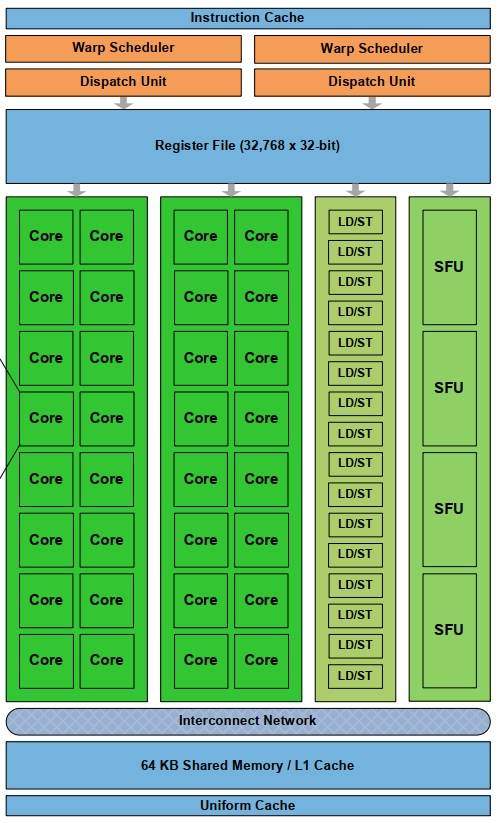
\includegraphics[width=0.4\linewidth]{picts/sm_nvidia}
	\caption{Архитектура видеокарты NVIDIA.}
	\label{fig:smnvidia}
\end{figure}
	%\textbf{\emph{Последовательный доступ}}. 
	\subsubsection*{Последовательный доступ}
	
	Потоки в ворпе обладают последовательными идентификаторами в коде ядра. Необходимо организовывать решение таким образом, чтобы запись и чтение данных этими потоками происходили в соседних ячейках памяти. Это связано с тем, что для каждого запроса к глобальной памяти выгружается непрерывная кеш-линия данных, и, если соседнему потоку нужны данные из этой же области памяти, она используется наиболее эффективно, иначе придется выгружать новую кеш-линию.
	
	%\textbf{\emph{Расхождение кода}}.
	\subsubsection*{Расхождение потоков}
	
	Работа потоков, находящихся в пределах одного ворпа, организована по принципу SIMD. Потоки делят один указатель на инструкцию, и если в коде есть ветвления, а соседние потоки удовлетворяют различным предикатам, то фактически все ветки будут исполнены ворпом последовательно. Если одна из веток требует значительно больших затрат на обработку, следует выносить такие вычисления в разные ядра, чтобы часть потоков не простаивала в ожидании.
	
	%\textbf{\emph{Обращение к глобальной памяти}}.
	\subsubsection*{Обращение к глобальной памяти}
	
	Потокам доступны несколько областей памяти, и обращения к глобальной памяти самые дорогие по времени. Если в ядре предполагается нетривиальная вычислительная работа и многократное использование данных, следует предварительно перенести данные в локальную память, обращения к которой в сотни раз быстрее. 
	
	\subsection{Библиотеки  операций с разреженными булевыми матрицами}\label{libs}
	
	Необходимость в операциях с разреженными матрицами возникла достаточно давно, и на данный момент достигнуты существенные успехи в разработке соответствующих алгоритмов. Некоторые операции были реализованы в библиотеках линейной алгебры в рамках стандарта BLAS. Такие библиотеки не предоставляют специальных версий алгоритмов для булевых матриц. Это является значимым недостатком, так как для булевой матрицы требуется меньше памяти и арифметических вычислений. Мы сравним библиотеки по следующим критериям:
	\begin{enumerate}[itemsep=0mm, topsep=0pt]
		\item[--] набор поддерживаемых операций,
		\item[--] технологии: CUDA, OpenCL, NVIDIA, OpenMP,
		\item[--] алгоритмы для сложения и умножения,
		\item[--] стандарт API.
	\end{enumerate}
	
	Полную реализацию стандарта GraphBlas с операциями над булевым полукольцом предоставляет библиотека SuiteSparse \cite{suite_sparse}. На данный момент разработчики библиотеки добавили поддержку OpenMP, также ведется активная работа над реализацией на CUDA при поддержке NVIDIA. Способы реализации тех или иных операций этой библиотекой нам малоинтересны, так как они не учитывают архитектуру видеокарты.
	
	Операции сложения и умножения можно найти в двух CUDA-ориентированных библиотеках: cuSPARSE и CUSP. cuSparse -- это проприетарная библиотека от NVIDIA с закрытым исходным кодом. Код CUSP находится в открытом доступе, а используемый алгоритм умножения опубликован \cite{dalton}. CUSP также содержит целиком реализованные алгоритмы на графах, представленных разреженными матрицами смежности: поиск в ширину, максимальное независимое множество и другие. Обе библиотеки работают и с плотными матрицами. 
	
	К OpenCL решениям относится библиотека clSPARSE, разработанная с поддержкой AMD, но в ней отсутствует одна из ключевых операций -- поэлементное сложение матриц. 
	
	Сравнение этих библиотек с нашим решением по потреблению времени и памяти будет приведено в \ref{experiments}-й главе работы. 
	
	
	\subsection{Форматы разреженных матриц}
	Все существующие форматы хранения разреженных матриц можно разделить на общие и специальные. Специальные форматы подходят для хранения матриц, структура которых заранее известна. Например, если в матрице большинство ненулевых элементов расположены на диагонали, хорошо подойдет диагональный формат. Мы будем ориентироваться на матрицы произвольной внутренней структуры, поэтому сосредоточимся на общих форматах. 
	
	Для начала введем некоторые обозначения, которыми принято описывать представление разреженной матрицы в сжатом формате:
	
	\begin{itemize}[itemsep=0mm, topsep=0pt]
		\item \txt{nnz} -- количество ненулевых элементов матрицы,
		\item \txt{nzr} -- количество строк матрицы с хотя бы одним ненулевым элементом,
		\item \txt{rows} -- массив строковых индексов,
		\item \txt{cols} --  массив столбцовых индексов,
		\item \txt{rpt} -- массив указателей на начала строк.
	\end{itemize}
	
	Самым простым форматом является координатный. В нём матрица хранится в виде списка пар – координат ненулевых элементов. Для удобства индексации элементы в парах упорядочены сначала по строкам, затем по столбцам. В памяти такой формат представлен двумя массивами – \txt{rows} и $cols$, каждый по $nnz$ элементов. Для матрицы $M_{m\times n}$ $k$-ый ненулевой элемент $M[i][j]$ будет сохранен в массивах как $(rows[k], cols[k]) = (i, j)$. Итого формат требует $2 * nnz * sizeof (index\_type)$ байт памяти. Индексация по строкам будет происходить за $O(log (nnz))$. Такой формат удобен для передачи матрицы в библиотеку.
	
	Самым популярным форматом для реализации операций с разреженными матрицами является CSR – compressed sparse row. В координатном формате можно заметить дублирование строковых индексов в количестве ненулевых элементов ряда. CSR сжимает эту информацию и вместо строковых индексов хранит массив \txt{rpt} (row pointers) c началом каждого ряда в массиве $cols$. Например, начало $i$-го ряда будет записано в ячейке $rpt[i]$. Индексация по строкам осуществляется за $O(1)$. За быструю индексацию мы платим тем, что храним в \txt{rpt} информацию о пустых рядах матрицы в том числе. Для матрицы $M_{m \times n}$ массив \txt{rpt} займет $(m + 1) * sizeof (index\_type)$ памяти. Итого формат требует $(nnz + m + 1) * sizeof (index\_type)$ байт. В CSR удобно вычислить длину $i$-го ряда как $rpt[i+1]-rpt[i]$, это пригодится для оценки вычислительной нагрузки на каждый ряд в ходе матричных операций. 
	Если отсортировать матрицу по строковым индексам и сделать сжатие по массиву $cols$, получится зеркальный к CSR формат CSC – compressed sparse column. 
	
	Заметим, что координатный формат занимает $O(nnz)$ памяти и это может быть преимуществом в случае матриц, в которых элементов значительно меньше, чем строк. Такие матрицы являются сверхразреженными, и для их хранения был предложен формат DCSR (DCSC) \cite{dcsr}. Если удалить информацию о пустых рядах из массива \txt{rpt} формата CSR, мы больше не знаем, какой ряд начинается в $rpt[i]$, следовательно, необходимо вернуть массив \txt{rows}. В таком формате индексация по строкам матрицы осуществляется за $O(log(nzr))$. Для ускорения индексации строковые индексы группируют по корзинам размера $n/nzr$. Вводится дополнительный массив \textit{AUX} размера $nzr$, хранящий указатели на начало каждой корзины. В случае равномерного распределения индексов непустых рядов, в каждой корзине будет в среднем один элемент. Если распределение смещено, то в корзине может быть до $n/nzr$ элементов. 
	
	Мы поставили перед собой задачу реализовать матричные алгоритмы, используя $O(nnz)$ памяти. Из всех операций только сложение матриц и произведение Кронекера осмысленно реализовывать в координатном формате.  Для остальных операций мы использовали формат DCSR. Преимуществом формата DCSR является его заменимость форматом CSR, так как их использование часто отличается  способом индексации рядов. 
	В таблице \ref{formats} приведено сравнение форматов по потребляемой памяти и времени индексации ряда для матрицы размером $m\times n$. 
		
		\begin{table}
			\centering
			\begin{tabular}{ |p{2.6cm} |p{3cm}|p{3cm}|p{3.5cm}| } 
				\hline
				       & COO & CSR & DCSR \\ 
				\hline
				Память & \makecell[tl]{ \txt{rows[nnz]} \\  + \txt{cols[nnz]} \\ = \txt{\bld{O(nnz)}}}
					   & \makecell[tl]{ \txt{rpt [m + 1]} \\ + \txt{cols[nnz]} \\ =  \txt{\bld{O(m, nnz)}}} 
					   & \makecell[tl]{ \txt{rpt [m + 1]} \\ + \txt{rows[m]} \\ + \txt{cols[nnz]} \\ + \txt{*AUX [nnz]} \\ = \txt{\bld{O(nnz)}}} \\ 
				\hline
				Индексация ряда  & \txt{O(log(nnz))} & \txt{O(1)} & \makecell[tl]{ \txt{O(log(nzr))} \\ *\txt{O(log(nnz/nzr))}} \\ 
				\hline
			\end{tabular}
			\caption{Сравнение форматов по занимаемой памяти и индексации для матрицы $M_{m\times n}$, * -- при добавлении массива AUX.}
			\label{formats}
		\end{table}
		
	В библиотеке нам будут интересны все три формата. Если алгоритмы для DCSR и CSR отличаются только индексацией ряда, то для COO методы будут реализованы по-другому, так как все его данные можно воспринимать как единый отсортированный массив, а не только как последовательность сортированных строк.
	
	
	\subsection{Основные идеи алгоритмов матричного умножения}
	
	Матричное умножение является частью большого числа алгоритмов и вычислений, особенно в линейной алгебре и анализе графов, что объясняет активное развитие алгоритмов в этой области. С появлением GPGPU начали развиваться подходы, опирающиеся на архитектуру видеокарт. Оказалось, что умножение разреженных матриц -- это непростая задача для модели массового параллелизма GPGPU, так как её нельзя разбить на равные по вычислительным затратам подзадачи. В данном разделе мы рассмотрим основные идеи, которые были предложены исследователями для адаптации матричного умножения под архитектуру GPU. 
	
	\subsubsection*{Формулировка матричного умножения}
	
	Классическая формулировка умножения матриц $A_{m\times k}$ и  $B_{k\times n}$ основана на скалярном произведении строк матрицы $A$ и столбцов матрицы $B$:
	
	$$c_{ij} = \sum_{l=1}^{k}a_{ik}*b_{kj}$$
	
	Такая формулировка требует быстрого доступа к строкам матрицы $A$ и столбцам матрицы $B$. В представлении форматов мы упоминали CSC, симметричный к CSR. Если хранить матрицы в разных форматах -- $A$ в CSR и $B$ в CSC, то можно добиться требуемого свойства, что и сделано на данный момент в библиотеке GraphBlast\cite{graphblast}. Недостатком подхода является затратная смена формата с CSR на CSC, так как она требует переупорядочивания индексов.
	
	Самая часто используемая для умножения разреженных матриц формулировка основана на формировании строк матрицы $C$ целиком, а не отдельных её значений:
	
	$$C[i,:]=\sum_{k\in nzr(A[i, :])}A[i, k] * B[k, :]$$
	
	Каждая строка матрицы $C$ -- это линейная комбинация строк матрицы $B$, с весом, взятым с соответствующей позиции ряда $A$. Такой подход описан ещё в работах 70-х годов \cite{gustavson}.  
	
	Для второй формулировки естественно использовать ориентированные на строки форматы, а именно CSR и DCSR. 
	
	\subsubsection*{Вычисление размера матрицы} 
	
	Конструирование новых строк матрицы \txt{C} в случае булевых матриц – это объединение нескольких строк матрицы \txt{B} с удалением повторяющихся значений. Предсказать заранее количество повторов невозможно, как и длину новой строки.
	
	Существуют два основных подхода к выделению памяти для процедуры умножения. 
	Первый подход предлагает создать достаточно большую временную матрицу $\tilde{C}$, в которую можно записывать результат слияния строк. Согласно второму подходу, промежуточная матрица не создается -- сначала выполняется символьное умножение, на этапе которого вычисляются длины новых строк, что позволяет выделить точное количество памяти для матрицы \txt{C}. 
	
	Выделить память на временную матрицу $\tilde{C}$ можно несколькими способами. Самый простой из них -- воспользоваться верхней границей. Верхняя граница длины строки матрицы $C$ -- это сумма длин входящих в неё строк из $B$.  Псевдокод подсчета ненулевых элементов в форматах CSR и DCSR без AUX-массива приведен в листингах 1 и 2. Отметим, что разница реализации всех алгоритмов для этих форматов будет заключаться в индексировании строк: для DCSR нам необходимо бинарным поиском найти позицию соответствующего ряда с помощью функции $search$.
			
\begin{minipage}{\linewidth}%
\small
\begin{lstlisting}[breaklines=true, basicstyle=\small, caption={Оценка размера ряда, формат DCSR}, style=mystyle]
nnz_est[global_id] = 0;
for (uint col_idx = a_rpt[global_id]; col_idx < a_rpt[global_id + 1]; ++col_idx) {
	uint col_ptr = a_cols[col_idx];
	uint col_ptr_pos = search(b_rows, col_ptr, b_nzr);
	if (col_ptr_pos == b_nzr) continue;
	nnz_est[global_id] += b_ptr[col_ptr_pos + 1] - b_ptr[col_ptr_pos];
}
\end{lstlisting}
\end{minipage}

\begin{minipage}{\linewidth}%
\small
\begin{lstlisting}[breaklines=true, basicstyle=\small, caption={Оценка размера ряда, формат CSR}, style=mystyle]
nnz_est[global_id] = 0;
for (uint col_idx = a_rpt[global_id]; col_idx < a_rpt[global_id + 1]; ++col_idx) {
	uint col_ptr = a_cols[col_idx];
	nnz_est[global_id] += b_ptr[col_ptr + 1] - b_ptr[col_ptr];
}
\end{lstlisting}
\end{minipage}

	Часто объем памяти, выделенный в соответствии с верхней оценкой, является избыточным. Поэтому можно воспользоваться \emph{прогрессивным} подходом – выделить сколько-то памяти для \textit{C}, и в случае нехватки запустить сложение заново с большим запасом памяти. Такой подход используется в MATLAB\cite{matlab}. 

	Существует \emph{гибридный} метод выделения памяти. На основе верхней оценки строки разбиваются на корзины с определенным порогом. Память выделяется так, что вычисление может закончиться неудачей только для самых больших корзин. В таком случае снова придется выделить новую б\emph{о}льшую матрицу $\tilde{C}$, в которую будет скопирован результат предыдущих вычислений. 
	Успешно вычислив матрицу $\tilde{C}$, выделяют точное количество памяти для матрицы $C$ и копируют полученные значения.
	
	\subsection*{Распределение нагрузки между потоками} 
	
	
	Балансировка работы потоков необходима для наиболее полного и эффективного использования мощностей вычислительного устройства. Иначе какие-то потоки быстро закончат свою работу и будут простаивать, пока другие группы работают над более сложными задачами.
	
	Одним из популярных подходов является формирование массива перестановок, определяющего, в каком порядке обрабатывать строки матрицы $A$. Такой подход реализован в библиотеке CUSP \cite{dalton}.
	
	Как мы говорили выше, ни один алгоритм не обходится без предварительной верхней оценки каждой строки матрицы $C$. Здесь эта оценка используется для распределения нагрузки на потоки. Создается массив перестановок \txt{P}, определяющий порядок вычисления строк матрицы \txt{C}. В результате строки будут выложенны в памяти непоследовательно, что является недостатком такого подхода.
	
	В двух наиболее популярных алгоритмах матричного умножения \cite{liu, nagasaka}, реализация которых в библиотеках линейной алгебры подтвердила их практическую значимость, этот массив используется для группировки строк матрицы $A$ по корзинам. Корзины можно обрабатывать одним и тем же способом, но выделить разное число потоков в зависимости от размера корзины, а можно и разными способами. 
	
	На большие и средние ряды выделяют рабочие группы разных размеров, тогда как маленькие ряды можно обрабатывать одним потоком. Паттерн доступа на чтение и запись для рядов, формируемых одним потоком, будет непоследовательным: два соседних потока могут читать данные из далеко расположенных ячеек глобальной памяти, что существенно влияет на производительность. Но эти потери компенсируются упорядоченной результирующей матрицей, а также временем работы ядер, формирующих большие ряды. 
	
	Далее мы рассмотрим два основных способа формировать ряды новой матрицы на примере алгоритмов В. Лю \cite{liu} и Ю. Нагасака \cite{nagasaka}. Оба алгоритма мы использовали для реализации умножения в нашей библиотеке.
	
	\subsection*{Формирование строк с помощью слияния, алгоритм В. Лю}
	
	В алгоритме В. Лю \cite{liu} строки будущей матрицы \txt{C} группируются в соответствии с верхней оценкой их размера, и каждая группа обрабатывается по-своему. Алгоритм опирается на отсортированные строковые индексы входных матриц и сразу формирует ряды новой матрицы в отсортированном порядке. 
	
	Упорядоченность входных матриц используется только для самых больших рядов. В случае, когда верхняя оценка длины строки равна 0 или 1, код вычислительного ядра тривиален. Для рядов до 32-х элементов используется пирамидальная сортировка: сначала массив в локальной памяти заполняется рядами матрицы \txt{B}, а затем сортируется. Удаление дубликатов происходит на последнем этапе сортировки: когда необходимо взять вершину пирамиды и записать к уже отсортированной части массива, достаточно проверить, что последний сохраненный там элемент не равен вершине. Если же он оказывается равен, вершина пирамиды извлекается без дальнейшей записи. Для формирования каждого ряда таким способом выделяется один поток.  
	
	Другой способ обработки применяется к группам со следующими оценками верхней границы: 33--64, 65--128, 129--256, 257--512. Разбиение внутри одного и того же способа обработки необходимо для распределения нагрузки на потоки. В отличие от предыдущей корзины, на каждый ряд выделяется не один поток, а рабочая группа, размер которой зависит от верхней оценки. Так же, как и в предыдущем методе, строки копируются в локальный массив, но затем к ним применяется битоническая сортировка, которая переставляет элементы на месте и задействует количество потоков, равное половине размера массива. После сортировки в массиве остаются повторяющиеся элементы, и они располагаются друг за другом. Подробное описание удаления дубликатов в упорядоченном массиве будет дано в разделе \ref{section:add}, так как это основа сложения матриц в координатном формате. 
	
	Строки размером от 512--ти элементов формируются постепенным слиянием строк. Из каждой новой строки матрицы \txt{B} в локальную память сохраняются только уникальные элементы, которых нет среди уже объединенных строк, а затем происходит слияние алгоритмом Merge Path \cite{green}. Как только ряд перестает помещаться в локальную память, результат сохраняется в глобальную память и процесс продолжается. 
	
	На финальном этапе выделяется память под матрицу \txt{C} и в неё копируются вычисленные элементы из \~{\txt{C}}.
	
	
	\subsection*{Формирование строк с помощью хэш-таблиц, алгоритм Ю. Нагасака}
	
	Алгоритм Ю. Нагасака \cite{nagasaka} также предполагает разделение строк на группы по верхней оценке количества ненулевых элементов. Для формирования всех строк используется хэш-таблицы с открытой адресацией, а группировка влияет на размер таблицы и её расположение в глобальной или локальной памяти. 
	
	Алгоритм является двухпроходным и состоит из символьной и численной частей. После символьной части известен точный размер финальной матрицы, а дополнительная глобальная память требуется только для обработки больших рядов. 
	
	При использовании хэш-таблиц строковые индексы оказываются неупорядоченными, поэтому на численном этапе элементы необходимо отсортировать. Авторы статьи в своей реализации используют сортировку подсчетом.    
	
\section{Реализация библиотеки операций с разреженными булевыми матрицами}
	
	
	В данном разделе подробно описаны реализации матричных операций. Для матричного умножения были реализованы алгоритмы В. Лю \cite{liu} и Ю. Нагасака \cite{nagasaka}, представленные в первой главе. Алгоритмы для остальных операций естественно следуют из формата матрицы.
	
	Далее мы представим библиотеку clBool\cite{clbool}, предоставляющую наши реализации.   
	
	\subsection{Описание и реализации операций} \label{details}
	
	Выбранные операции требуется реализовать над булевым полукольцом. Из этого следует, что операция сложения $"+"$ определена как $"\lor"$, а умножение $"*"$ определено как $"\land"$.
	
	В тех операциях, где требуется обработка строк, неэффективно использовать формат \textit{COO}. Однако особенность его структуры, а именно представление матрицы как единого упорядоченного массива пар, можно использовать для сложения, произведения Кронекера и транспонирования.
	
	\subsubsection{Умножение матриц}
	
	В первой главе мы рассмотрели основные идеи алгоритмов умножения матриц, а также рассказали про два алгоритма, которые сочетают в себе наиболее удачные из идей, но имеют существенные отличия в способе формирования итоговой матрицы и обработке строк.
	
	Оба алгоритма разработаны для CSR формата. Изменения, необходимые для перехода на формат DCSR, связаны с индексацией строк внутри ядра и с формированием массивов \txt{rpt} и \txt{rows}. Индексация осуществляется бинарным поиском по строкам, а в массивах \txt{rpt} и \txt{rows} нужно дополнительно следить за отсутствием пустых рядов.
	
	Алгоритм В. Лю отличается большим числом ядер, реализации которых слабо связаны между собой. Особого внимания заслуживает способ обработки самых больших рядов. В локальной памяти выделяется массив, в который постепенно сливают строки, и, как только память кончается, результат копируется в глобальную память. Если локальный массив вновь оказывается полностью заполненным, его необходимо соединить с тем, что уже лежит в глобальной памяти. Параллельное слияние возможно только с выделением дополнительных ресурсов глобальной памяти, помимо промежуточной матрицы \~{\txt{C}}, которая была аллоцирована с запасом.  
	
	Алгоритм Ю. Нагасака был опубликован на 5 лет позже. За это время изменились характеристики видеокарт, и в алгоритме активно используется возможность создавать большие воркгруппы до 1024 потоков. Также предлагается обрабатывать в локальной памяти хэш-таблицы до 8192 элементов. Мы ограничили размер воркгруппы до 256 для видеокарт AMD, а также максимальный размер хэш-таблицы до 4096, что привело к другим разбиениям строк для обработки.
	 
	Все ядра алгоритма эксплуатируют идею хэш-таблиц, что делает их сильно схожими в реализации. На последнем этапе в части ядер происходит сортировка хэш-таблицы. Авторы в своей реализации используют сортировку подсчётом с атомарными операциями, являющимися точками синхронизации. Мы выбрали битоническую сортировку, так как она сортирует массив на месте и хорошо подходит для параллельной обработки. 
	
	Мы не стали выносить группировку рядов на видеокарту. Задача группировки активно опирается на атомарные операции, которые являются по сути точкой синхронизации.  
	 
	В главе \ref{experiments} мы сравним эффективность обоих алгоритмов. 
	 
	\subsubsection{Сложение матриц}\label{section:add}
	
	\begin{figure}
		\centering
		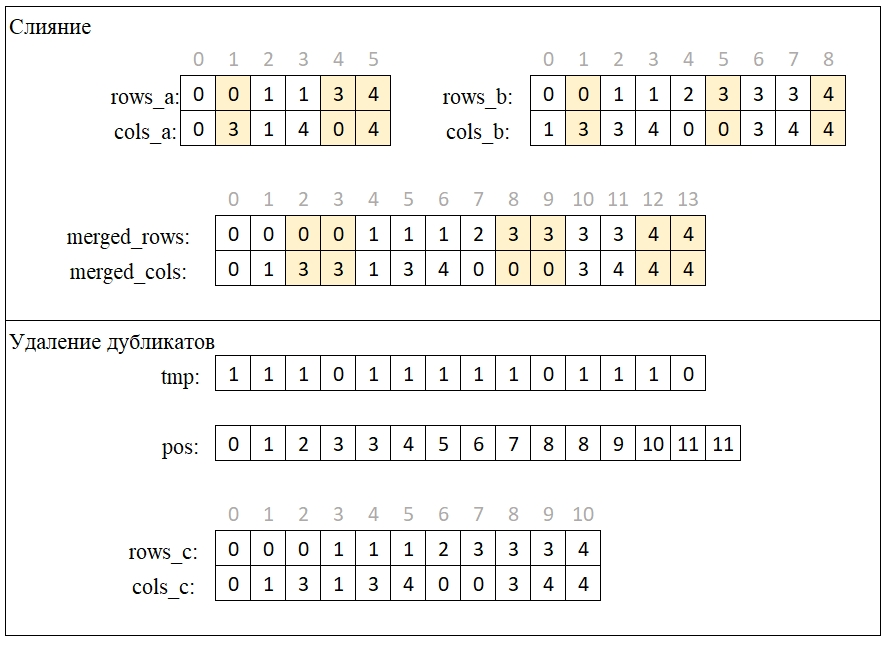
\includegraphics[width=0.8\linewidth]{picts/addition}
		\caption{Сложение в координатном формате.}
		\label{addition}
	\end{figure}
	
	
	В формате \textit{COO}, где каждая матрица является упорядоченным списком пар, сложение -- это слияние двух отсортированных списков. По сравнению со слиянием строк в умножении, размер конечного списка известен с большей точностью -- он не превысит суммы длин входных матриц. 
	
	Пример сложения представлен на рисунке \ref{addition}.  Для удаления дубликатов формируется временный массив $tmp$, в котором значение “1” стоит на позиции элементов, не повторяющих предыдущий. Массив $pos$ -- это префиксная сумма по массиву $tmp$ без включения, то есть элемент на позиции $i$ вносит свой вклад в значение префиксной суммы на позиции $i + 1$. Таким образом, если $pos[i] = pos[i + 1]$, значение в исходном массиве на позиции $i$ является чьим-то дубликатом и его не нужно записывать результат. Если же $pos[i] \neq pos[i + 1]$, то $pos[i]$ является новой позицией уникального элемента из исходного массива.
	
	В последнем элементе массива $pos$ аккумулируется значение, равное количеству всех уникальных ненулевых элементов. Так мы узнаем, сколько точно нужно выделить памяти для финальной матрицы.
	
	Параллельное слияние реализовано с помощью алгоритма Merge Path \cite{green} с использованием локальной памяти. 
	 
	Сложение в форматах CSR и DCSR основано на той же последовательности действий, примененной к каждой строке. Слияние и префиксную сумму можно реализовать в локальной памяти, постепенно обрабатывая ряд фрагментами, которые туда помещаются. В случае CSR и DCSR форматов имеет смысл разделить сложение на символьную и численную части. На первом этапе вычисляется размер каждого ряда новой матрицы, что позволяет сразу выделить точное количество памяти. На втором этапе можно осуществлять запись в подготовленный массив.  
		
	\subsubsection{Произведение Кронекера}\label{kron}
	
	
	\emph{Произведение Кронекера} обозначают как $С = A\otimes B$. Для входных матриц $A_{m_1 \times n_1}$ и $B_{m_2 \times n_2}$ результатом является матрица $C$ следующего вида:
	
	$$
	A\otimes B = \begin{pmatrix}
		
		a_{11}b_{11} & \dots & a_{11}b_{1n_2} & \dots & a_{1n_1}b_{11} & \dots & a_{1n_1}b_{1n_2}\\
		\vdots & \ddots & \vdots & \dots & \vdots & \ddots & \vdots \\
		a_{11}b_{m_{2}1} & \dots & a_{11}b_{m_2n_2} & \dots & a_{1n_1}b_{m_{2}1} & \dots & a_{1n_1}b_{m_2n_2}\\
		\dots & \dots & \dots & \dots & \dots & \dots & \dots \\
		a_{m_{1}1}b_{11} & \dots & a_{11}b_{1n_2} & \dots & a_{1m_1}b_{11} & \dots & a_{m_1n_1}b_{1n_2}\\
		\vdots & \ddots & \vdots & \dots & \vdots & \ddots & \vdots \\
		a_{m_1n_1}b_{m_{2}1} & \dots & a_{m_1n_1}b_{m_2n_2} & \dots & a_{m_1n_1}b_{m_{2}1} & \dots & a_{m_1n_1}b_{m_2n_2}\\
	\end{pmatrix}$$
	
	Если $C = A\otimes B$, то $C[i_1 * m_2 + i_2, j_1 * n_2 + j_2] = A[i_1, j_1] * B[i_2, j_2]$.
	
	Для формата DCSR первым шагом необходимо рассчитать массивы указателей \txt{rpt} и \txt{rows}. Массив \txt{rpt} формируется стандартным способом -- сначала считаем размер каждого ряда, а затем вычисляем префиксную сумму без включения. Для данного шага достаточно выделить $nzr(A) * nzr(B)$ потоков, каждый из которых определит, к каким строкам матриц $A$ и $B$ относится его ряд и сохранит произведение их длин.  
	
	Для вычисления столбцовых индексов выделим $nnz(A) * nnz(B)$ потоков, где каждый поток запишет один индекс.
	
	Иначе можно вычислить произведение Кронекера, если матрицы представлены в формате COO. Вместо того чтобы формировать матрицу в упорядоченном виде, запишем индексы, группируя по матрицам $B$. Тогда координаты оказываются полностью вычислены за один шаг, но результат требует сортировки.
	
	Полученная в результате произведения Кронекера матрица оказывается довольно большой, и часто координатное представление избыточно и затратно по памяти. 
	
	\subsubsection{Редуцирование строк матрицы}
	
	\emph{Редуцирование матрицы} $A_{m\times n}$ по строкам -- это матрица $M_{m\times 1}$, для которой $M[i,0] = 1$ если в исходной матрице строка $i$ содержала хотя бы одно ненулевое значение.
	
	Это несложная операция для формата DCSR. В массиве \txt{rows} перечислены только непустые ряды, поэтому он полностью копируется. Изменения в массивах \txt{cols} и \txt{rpt} представлены в листинге \ref{reduce}.
	
	\begin{minipage}{\linewidth}%
		
\begin{lstlisting}[breaklines=true, basicstyle=\small, caption={Массивы rpt и cols при редуцировании матрицы}, label={reduce}]
cols[global_id] = 0;
rpt[global_id] = global_id;
		\end{lstlisting}
	\end{minipage}
	
	
	\subsubsection{Извлечение подматрицы}
	
	\emph{Извлечение подматрицы} -- это операция с параметрами $i, j, ncols, nrows$, результатом которой является подматрица $M_{ncols \times nrows}$ исходной матрицы, строки и столбцы которой начинаются с позиций $i$ и $j$ исходной матрицы. 
	
	
	Вычисление подматрицы состоит из двух этапов: определение размера результата и заполнение индексов подматриц. Сначала необходимо определить позиции строк подматрицы в массиве \txt{rows}. Затем вычисляются позиции столбцовых индексов для каждой строки. Поиск нужных индексов строк и столбцов в формате DCSR осуществляются бинарным поиском. Полученный массив \txt{rows} является для подматрицы временным, так как после выделения нужных столбцов некоторые строки будут пустыми.
	
	Запись строк может осуществляться как с группировкой, так и без неё. Удаление пустых строк повторяет процесс удаления дубликатов при сложении матриц. 
	
	
	\subsubsection{Транспонирование}
	
	Для формата COO транспонирование заключается в перестановке местами данных массивов \txt{rows} и \txt{cols} c последующей сортировкой индексов. Реализовать транспонирование для DCSR удобно через конвертацию между форматами. В COO и DCSR массив \txt{cols} полностью совпадает, требуется только формировать массивы \txt{rows} и \txt{rpt}.  
	
	
	\sectionbreak
	
	\subsection{Библиотека clBool}
	
	
	Библиотека clBool написана на языке C++17. Для её работы необходимо устройство, поддерживающее стандарт OpenCL 1.1 с установленным окружением, которое можно найти на сайте вендора. Выбор стандарта 1.1 обусловлен тем, что карты NVIDIA не поддерживают стандарты 2.x. 
	
	\subsubsection*{Структура библиотеки}
	
	Структура библиотеки представлена на рисунке \ref{clboolarc}. Компоненты отображают файловую структуру исходного кода. 
	

	\begin{figure}
		\centering
		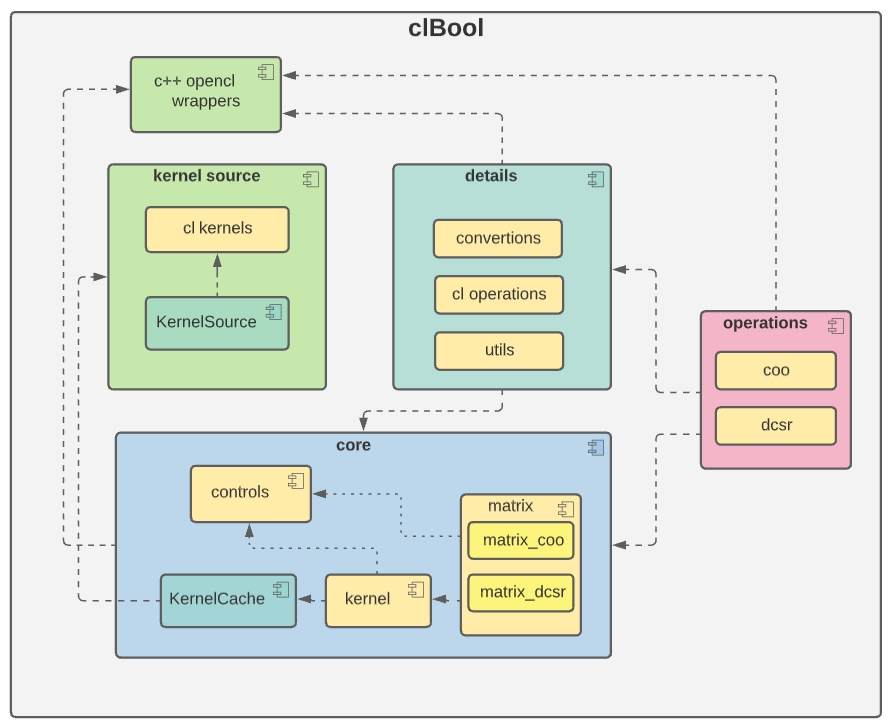
\includegraphics[width=0.8\linewidth]{picts/clBool_cmps}
		\caption{Компоненты clBool.}
		\label{clboolarc}
	\end{figure}
	 
	
	Ядро содержит набор классов, необходимых для организации внутренней работы библиотеки.

	Состояние библиотеки содержится в классе \textbf{Controls}. Экземпляр класса передается во все вызовы библиотеки, из него доступны необходимые для OpenCL объекты: выбранное устройство, контекст и очередь задач. 
	  
	Матрицы представлены классами \textbf{matrix\_coo} и \textbf{matrix\_dcsr}. Они хранят массивы индексов в памяти выбранного устройства, а также основную информацию о матрице: размер, количество ненулевых элементов, количество непустых строк (для DCSR).
	
	Класс \textbf{kernel} отвечает за загрузку и исполнение ядра на видеокарте. Компиляция программ для видеокарты происходит во время исполнения основной программы. Чтобы не работать с чтением данных из файла, код хранится в статических переменных заголовочных файлов, которые генерируются во время сборки. На видеокартах AMD первая компиляция ядра длится значительно дольше его исполнения. Поэтому мы храним скомпилированные однажды программы в статических полях класса \bld{KernelCache}.
	
	В блоке \bld{details} собраны функции, которые часто используются при работе с обоими форматами, например, конвертации между форматами и префиксная сумма массива. Также этот блок содержит набор макросов для логирования, позволяющих в режиме дебага сохранять время исполнения всех промежуточных этапов алгоритмов. 
	
	Блок \bld{operations} содержит реализации матричных операций, собранные в пространствах имен соответствующих форматов.
	
	\subsubsection*{Управление ресурсами}
	
	Для управления ресурсами OpenCL используются C++-обертки от Khronos Group \cite{khronos_wrap}, которые являются в том числе разработчиками стандарта. Заголовочный файл \emph{opencl.hpp} импортирует RAII\footnote{RAII -- захват ресурса есть инициализация -- программная идиома, согласно которой создание и освобождение ресурса связано с инициализацией и удалением объекта.} обертки над ресурсами: буфером, программой, очередью, девайсом, событием, что позволяет перенаправить задачу управления памятью на объект -- владельца ресурса. 
	
	\subsubsection*{Обработка вызовов}
	
	Для инициализации состояния библиотеки требуется указать устройство, на котором должны исполняться ядра. В OpenCL каждое устройство соответствует платформе, поэтому для его идентификации требуется два индекса: платформы и устройства. Список доступных платформ и устройств с идентификаторами можно вывести функцией $show\_devices$. По умолчанию используется устройство с минимальным идентификатором. 
	
	Пример поэлементного сложения матриц средствами библиотеки clBool представлен в Листинге \ref{example}.
	
\begin{minipage}{\linewidth}%
	\small
	\begin{lstlisting}[breaklines=true,caption={Инициализация состояния и вызов функции сложения}, label={example}, style = mystyle]
clbool::Controls controls = clbool::create_controls(1, 0);
<@\textcolor{cmnt-color}{// данные для матрицы A}@>
uint32_t a_nrows = 5, a_ncols = 5, a_nnz = 6;
std::vector<uint32_t> a_rows = {0, 0, 0, 2, 2, 4};
std::vector<uint32_t> a_cols = {0, 1, 4, 2, 3, 2};
<@\textcolor{cmnt-color}{// данные для матрицы B}@>
uint32_t b_nrows = 5, b_ncols = 5, b_nnz = 7;
std::vector<uint32_t> b_rows = {1, 1, 2, 3, 3, 3, 5};
std::vector<uint32_t> b_cols =  {0, 4, 2, 2, 3, 4, 2};
<@\textcolor{cmnt-color}{// инициализация матриц}@>
clbool::matrix_coo a_coo(controls, a_nrows, a_ncols, a_nnz, a_rows.data(), a_cols.data());
clbool::matrix_coo b_coo(controls, b_nrows, b_ncols, b_nnz, b_rows.data(), b_cols.data());
<@\textcolor{cmnt-color}{// вызов функции сложения}@>
clbool::matrix_coo c_coo;
clbool::coo::matrix_addition(controls, c_coo, a_coo, b_coo);
\end{lstlisting}
\end{minipage}
	
	
\sectionbreak

\section{Экспериментальное исследование библиотеки}\label{experiments}
	
	В данной главе мы исследуем производительность наших реализаций матричных операций. 
	
	Сначала мы сравним две реализации произведения Кронекера, адаптированные под разные форматы хранения матриц. Затем мы сосредоточимся на двух самых затратных операциях, присутствующих в большинстве библиотек линейной алгебры -- поэлементное сложение матриц и умножение матриц. Мы сравним исполнение на различных устройствах, поддерживающих OpenCL: NVIDIA, AMD, FPGA, подробная характеристика которых представлена в таблице \ref{table:devs}, а также  сравним наши реализации с реализациями в популярных библиотеках линейной алгебры.
	
	\begin{table} 
		\centering
		\scriptsize
		\rowcolors{2}{black!2}{black!10}
		\small
		\begin{tabular}{ |p{2.1cm} |p{3cm}|p{2cm}|p{2cm}|p{2cm}|p{1.7cm}|} 
			\hline 
			Устройство & Полное имя  & Объем глобальной памяти, gb  & Объем локальной памяти, kb & Макс. размер рабочей группы & Тактовая частота, MHz\\ \hline 
			NVIDIA & GeForce GTX 1070 & 7.926 & 48 & 1024 & 1746 \\ \hline
			AMD &  Radeon Vega Frontier Edition & 15.98 & 64 & 256 & 1600  \\ \hline
			FPGA &  10AX115S2F45E2LG, Euler Line SODIMM Final & 
			8 & 16 & 2147483647 & 1000 \\ \hline
	

		\end{tabular}
		\caption{Характеристики устройств, используемых для экспериментов.}
		\label{table:devs}
	\end{table} 
	 
	
	\subsection{Произведение Кронекера: сравнение алгоритмов}
	
	Результатом произведения Кронекера является матрица, количество ненулевых элементов в которой равно произведению этих параметров у входных матриц. Следовательно, как только в вычислениях появляется произведение Кронекера, потребление видеопамяти резко возрастает.
	
	Как было сказано в \ref{kron}, реализации данной операции для форматов COO и DCSR существенно отличаются. Произведение Кронекера для формата COO содержит одно ядро для вычисления индексов и последующую их сортировку. В формате DCSR операция состроит из б\emph{о}льшего числа ядер, включающих вычисление префиксной суммы. 
	
		\begin{table}
		\centering
		\scriptsize
		\rowcolors{2}{black!2}{black!10}
		\small
		\begin{tabular}{ |c|r|r|c c|c c|} 
			\hline 
			№ & nnz(M)  & \multicolumn{1}{c|}{Размер}   & \multicolumn{2}{c|}{DCSR} & \multicolumn{2}{c|}{COO} \\ \cline{4-7} 
			M &       & \multicolumn{1}{c|}{результата}  & ms & mb & ms & mb \\ \hline
			1 & 1 000 & 1 000 000 & 0.77 & 97 & 3.15 & 93 \\ \hline
        	2 & 2 000 & 4 000 000 & 2.50 & 129 & 14.56 & 117 \\ \hline
        	3 & 3 000 & 9 000 000 & 5.23 & 177 & 52.25 & 157 \\ \hline
        	4 & 4 000 & 16 000 000 & 8.99 & 231 & 66.05 & 209 \\ \hline
        	5 & 5 000 & 25 000 000 & 13.36 & 301 & 128.76 & 277 \\ \hline
        	6 & 6 000 & 36 000 000 & 19.05 & 383 & 246.18 & 361 \\ \hline
        	7 & 7 000 & 49 000 000 & 25.18 & 469 & 278.83 & 461 \\ \hline
        	8 & 8 000 & 64 000 000 & 31.97 & 567 & 319.79 & 577 \\ \hline
        	9 & 9 000 & 81 000 000 & 36.32 & 659 & 562.47 & 705 \\ \hline
        	10 & 10 000 & 100 000 000 & 45.38 & 775 & 615.95 & 849 \\ \hline

			
		\end{tabular}
		\caption{Произведение Кронекера.}
		\label{table:kron}
	\end{table} 
	
	Для тестирования мы исполняли операцию $M\otimes M$ на случайных матрицах, постепенно увеличивая их заполненность. В качестве устройства выбрана видеокарта NVIDIA. 
	
	На небольших матрицах COO немного экономнее по памяти, это может быть связано с отсутствием вычисления префиксной суммы, которая требует дополнительной памяти. С увеличением наполненности матрицы COO начинает потреблять больше памяти за счёт двух массивов размера \txt{nnz}, из которых он состоит. Напомним, что формат DCSR содержит только один массив размер \txt{nnz} и два массива на \txt{nzr} элементов, где \txt{nnz} --  число ненулевых значений матрицы, а \txt{nzr} -- количество непустых строк.
	
	По времени исполнения существенно выигрывает реализация для формата DCSR. Самая дорогая операция в ядрах реализации -- это индексация строк и их элементов, на которую каждый поток тратит не более логарифма от размеров входных матриц. Сортировка, используемая для координатного формата, требует $O(\frac{n\log{n}^2} {\# ALU})$, где $n$ -- это количество ненулевых элементов в результирующей матрице, \txt{\# ALU} -- количество вычислителей на видеокарте. 
	
	По результатам замеров можно сделать вывод, что реализация произведение Кронекера для формата DCSR значительно более эффективна, чем реализация для формата COO.
	
	\subsection{Данные для тестирования сложения и умножения}
		
		Далее мы будем сравнивать производительность самых затратных матричных операций -- поэлементное сложение и матричное умножение. 
				\begin{table}
			\centering
			\small
			\rowcolors{2}{black!2}{black!10}
			\begin{tabular}{ |c|l|r|r|r|r|r|} 
				\hline
				№ & Имя & Размерность & $Nnz$ & \makecell[tc] {$Max$ \\ $nnz / row$}  & $Nnz(M^2)$ & $Nnz (M + M^2)$  \\
				\hline
				1 & wing & 62 032 & 243 088 & 4 &714 200 & 917 178 \\
				\hline
				2 & luxembourg\_osm & 114 599 & 239 332 & 6 & 393 261 & 393 261 \\ 
				\hline
				3 & amazon0312 & 400 727 & 3 200 440 & 10 & 14 390 544 & 14 968 909 \\ 
				\hline		
				4 & amazon-2008 & 735 323 & 5 158 388 & 10 & 25 366 745 & 26 402 678 \\ 
				\hline
				5 & web-Google & 916 428 & 5 105 039 & 456 & 29 710 164 & 30 811 855 \\ 
				\hline
				6 & roadNet-PA & 1 090 920 & 3 083 796 & 9 & 7 238 920 & 9 931 528  \\ 
				\hline
				7 & roadNet-TX & 1 393 383 & 3 843 320 & 12 & 8 903 897 & 12 264 987 \\ 
				\hline
				8 & belgium\_osm & 1 441 295 & 3 099 940 & 10 & 5 323 073 & 8 408 599 \\ 
				\hline
				9 & roadNet-CA & 1 971 281 & 5 533 214 & 12 & 12 908 450 & 17 743 342 \\ 
				\hline
				10 & netherlands\_osm & 2 216 688 & 4 882 476 & 7 & 8 755 758 & 13 626 132 \\ 
				\hline
				
			\end{tabular}
			\caption{Описание матриц.}
			\label{table:mdata}
		\end{table}
		
		Для замеров были выбраны сильно разреженные матрицы из коллекции SuiteSparse \cite{ssp_matrices}, отличающиеся плотностью ненулевых элементов и размерами. Матрицы описывают совершенно разные данные: связанные покупки в интернет-магазинах, веб-соединения, дорожные сети. 
		
		Для тестирования сложения мы выбрали выражение $M + M^{2}$, для умножения -- $M^{2}$. В сложении матрица $M^2$ вычислена заранее. В качестве GPU была использована видеокарта NVIDIA GeForce GTX 1070 GPU с 8 Gb RAM, процессор Intel Core i7-6700 CPU, 3.40Hz, DDR4 64Gb RAM.  
		
		Характеристики матриц а также размеры результатов операций представлены в таблице \ref{table:mdata}. 
		

	
	\subsection{Исполнение операций на AMD}
	
	Выбор стандарта OpenCL позволяет использовать видеокарты AMD. В нашем распоряжении была видеокарта AMD Radeon Vega Frontier Edition с 16Gb RAM. Мы запустили одни и те же алгоритмы, выбрав при инициализации библиотеки различные устройства. 
	
		\begin{table}
		\centering
		\rowcolors{2}{black!2}{black!10}
		\small
		\begin{tabular}{ |c|r r|r r|} 
			\hline
			M & \multicolumn{2}{c|}{$M^2$, ms} & \multicolumn{2}{c|}{$M+M^2$, ms} \\
			№ & AMD  & NVIDIA &  AMD  & NVIDIA  \\
			\hline
			1 & 2.10  & 1.29  & 1.71   & 1.73 \\ % 1.  wing             
			2 & 2.36  & 1.66  & 1.32   & 1.20 \\ % 2.  luxembourg\_osm  
			3 & 38.05 & 54.72 & 11.43  & 19.84 \\ % 3.  amazon0312       
			4 & 54.71 & 84.29 & 17.18  & 35.24 \\ % 4.  amazon-2008      
			5 & 86.20 & 125.53 & 19.34  & 38.10 \\ % 5.  web-Google       
			6 & 19.47 & 14.52 & 7.91  & 13.24 \\ % 6.  roadNet-PA       
			7 & 23.34 & 16.82 & 9.01  & 15.48 \\ % 7.  roadNet-TX       
			8 & 23.51 & 16.86 & 6.78  & 9.85 \\ % 8.  belgium\_osm     
			9 & 29.24 & 23.50 & 11.89  & 21.01 \\ % 9.  roadNet-CA       
			10 & 30.81 & 25.01 & 9.27  & 15.51 \\ % 10. netherlands\_osm  
			\hline
			
			
		\end{tabular}
		\caption{Сравнение AMD и NVIDIA.}
		\label{table:AMD}
	\end{table}
	
	Отметим, что видеокарта AMD обладает б\emph{о}льшим объемом локальной и глобальной памяти, чем карта NVIDIA. Это могло сказаться на результатах матричного сложения -- операция на AMD выполняется почти в 2 раза быстрее. На всех матрицах, кроме 3--5, лидирует исполнение на NVIDIA. Это связано с тем, что некоторые ядра ориентированы под размер ворпа равный 32-м потокам, тогда как на в ворпах видеокарт AMD 64 потока. Тем не менее, на матрицах с большим размером результата AMD работает стабильнее, что может объясняться большим объемом локальной памяти, которая активно используется в операции умножения.

	\subsection{Сравнение с библиотеками линейной алгебры}
	
	
	Мы будем сравнивать наши реализации с библиотеками, представленными в \ref{libs}, а также с реализациями матричных операций Артема Хорошева, обозначенными в таблицах как cuBool \cite{cubool}. Мы сможем более подробно сравниться именно с cuBool, так как нам известны детали этого решения. 
	
	\begin{table}
	\centering
	\rowcolors{2}{black!2}{black!10}
	\scriptsize
	\begin{tabular}{ |c|r r|r r|r r|r r|r r|r r|r r|} 
		\hline
		M  & \multicolumn{2}{c|}{cuBool} & \multicolumn{2}{c|}{clBool (1)} & \multicolumn{2}{c|}{clBool (2)} &
		 \multicolumn{2}{c|}{CUSP} &  \multicolumn{2}{c|}{cuSPRS} & 
		  \multicolumn{2}{c||}{clSPRS} & \multicolumn{2}{c|}{SuiteSparce}\\
		 № & ms  & mb &  ms  & mb  &  ms  & mb &  ms  & mb &  ms  & mb  &  ms  & mb &  ms  & mb \\
		\hline
		1 & 1.9 & 93 & 1.29  & 89 & 4.09 & 95 & 5.2  & 125 & 20.1 & 155 & 4.2 & 105 & 7.9  & 22  \\ % wing
	 	2 & 2.4  & 91  & 1.66   & 89  & 4.37 & 91 & 3.7   & 111  & 1.7    & 151 & 6.9   & 97   & 3.1   & 169 \\ % luxembourg_osm
		 3 & 23.2 & 165 & 54.72  & 163 & 58.81 & 273 & 108.5 & 897  & 412.8  & 301 & 52.2  & 459  & 257.6 & 283 \\ % amazon0312
		 4 & 33.3 & 225 & 84.28  & 221 & 95.70 & 401 & 172.0 & 1409 & 184.8  & 407 & 77.4  & 701  & 369.5 & 319 \\ % amazon-2008
		 5 & 41.8 & 241 & 125.53 & 239 & OOM & OOM & 246.2 & 1717 & 4761.3 & 439 & 207.5 & 1085 & 673.3 & 318 \\ % web-Google
		6 & 18.1 & 157 & 14.52  & 153 & 31.39 & 199 & 42.1  & 481  & 37.5   & 247 & 56.6  & 283  & 66.6  & 294 \\ % roadNet-PA
		 7 & 22.6 & 167 & 16.83  & 165 & 38.85 & 217 & 53.1  & 581  & 46.7   & 271 & 70.4  & 329  & 80.7  & 328 \\ % roadNet-TX
		 8 & 23.2 & 151 & 16.86  & 159 & 37.39 & 181 & 32.9  & 397  & 26.7   & 235 & 68.2  & 259  & 56.9  & 302 \\ % belgium_osm
		 9 & 32.0 & 199 & 23.50  & 211 & 53.98 & 271 & 74.4  & 771  & 65.8   & 325 & 98.2  & 433  & 114.5 & 344 \\ % roadNet-CA
		 10 & 35.3 & 191 & 25.00  & 189 & 55.85 & 261 & 51.0  & 585  & 51.4   & 291 & 102.8 & 361  & 90.9  & 311 \\ % netherlands_osm
		 \hline
 
	\end{tabular}
	\caption{Матричное умножение.}
	\label{table:mult}
	\end{table}
	
	
	Результаты замеров матричного умножения приведены в таблице \ref{table:mult}. Библиотека clBool представлена двумя реализациями операции: реализация, основанная на алгоритме Ю. Нагасака -- clBool (1) и В. Лю -- clBool (2). Решения на GPU ожидаемо выигрывают по времени у CPU-библиотеки SuiteSparse. Все библиотеки заметно падают в производительности на матрицах 3--5. Как видно в описании данных в таблице \ref{table:mdata}, результат умножения для этих матриц содержит большое число ненулевых элементов, а матрица 5 также имеет особо плотные ряды. 
	
	Такие матрицы существенно влияют на производительность операции в библиотеке cuSPARSE, где, вероятно, изначально выделяют меньше памяти на результат, чтобы в случае неудачи запустить вычисления ещё раз. Можно заметить, что в остальных строках таблицы cuSPARSE использует меньше памяти, чем другие библиотеки, что согласуется с гипотезой о переаллокации. Так как это библиотека с закрытым исходным кодом, мы не можем точно утверждать, как именно реализована операция.
	
		\begin{table}
		\centering
		\rowcolors{2}{black!2}{black!10}
		\small
		\begin{tabular}{ |c|r r|r r|r r|r r|r r||r r|} 
			\hline
			M & \multicolumn{2}{c|}{cuBool} & \multicolumn{2}{c|}{clBool} & 
			\multicolumn{2}{c|}{CUSP} &  \multicolumn{2}{c|}{cuSPRS} & 
			\multicolumn{2}{c||}{clSPRS} & \multicolumn{2}{c|}{SuiteSparce}\\
			№ & ms  & mb &  ms  & mb  &  ms  & mb &  ms  & mb &  ms  & mb  &  ms  & mb \\
			\hline
			1 & 1.1 & 95 & 1.73 & 105 & 1.4 & 105 & 2.4 & 163 & - & - & 2.3 & 176 \\ % 1.  wing             
			2 & 1.7 & 95 & 1.21  & 109 & 1.0  & 97 & 0.8 & 151 & -  & - & 1.6& 174 \\ % 2.  luxembourg\_osm  
			3 & 11.4 & 221 & 19.84  & 543 & 16.2 & 455 & 24.3 & 405 & - & - & 37.2 & 297 \\ % 3.  amazon0312       
			4 & 17.5 & 323 & 35.24  & 877 & 29.5 & 723 & 27.2 & 595 & - & - & 64.8 & 319 \\ % 4.  amazon-2008      
			5 & 24.8 & 355 & 38.09  & 989 & 31.9 & 815 & 89.0 & 659 & - & - & 77.2 & 318 \\ % 5.  web-Google       
			6 & 16.9 & 189 & 13.23  & 359 & 11.2 & 329 & 11.6 & 317 & - & - & 36.6 & 287 \\ % 6.  roadNet-PA       
			7 & 19.6 & 209 & 15.48  & 429 & 14.5 & 385 & 16.9 & 357 & - & - & 45.3 & 319 \\ % 7.  roadNet-TX       
			8 & 19.5 & 179 & 9.85  & 321 & 10.2 & 303 & 10.5 & 297 & - & - & 28.5 & 302 \\ % 8.  belgium\_osm     
			9 & 30.5 & 259 & 21.0  & 579 & 19.4 & 513 & 20.2 & 447 & - & - & 65.2 & 331 \\ % 9.  roadNet-CA       
			10 & 30.1 & 233 & 15.51  & 457 & 14.8 & 423 & 18.3 & 385 & -  & -   & 50.2 & 311 \\ % 10. netherlands\_osm  
			\hline
			
			
		\end{tabular}
		\caption{Поэлементное матричное сложение.}
		\label{table:add}
	\end{table}
	
	cuBool, clBool(1) и clBool(2) ожидаемо требуют меньше памяти по сравнению с  другими библиотеками, и справляются с операцией быстрее за счет отсутствия вычислений значений матрицы.
	
	Реализации cuBool и clBool (1) используют один алгоритм умножения на основе хэш-таблиц. Различия заключаются в подходе к группировке рядов и в формате матриц. В cuBool группировка полностью происходит на видеокарте и содержит много точек синхронизации, тогда как в clBool она вынесена на процессор. Основой библиотеки clBool является формат DCSR, а cuBool и остальных библиотек -- CSR. Также в отличается максимальный размер рабочей группы: до 1024 потоков в cuBool и 256 в clBool.  
	
	Наша реализация clBool (2) оказалась менее удачной по сравнению с cuBool и clBool (1). Использование промежуточной матрицы большого размера существенно влияет на потребление памяти. clBool (2) также уступает по времени исполнения, что можно объяснить недостаточным использованием ресурсов локальной памяти. 
	
	Во всех строках, кроме 3--5, реализация clBool оказывается быстрее cuBool. Возможно, именно способ группировки дает улучшение по времени на многих матрицах. Реализация cuBool оказалась устойчива к плотным матрицам. Заметим, что использование DCSR не дает существенных улучшений по потреблению памяти и скорее всего из-за логарифмической индексации строк clBool уступает cuBool по времени исполнения на плотный матрицах.
	
	Результаты замеров сложения матриц представлены в таблице \ref{table:add}. Все библиотеки, кроме cuBool, показывают сопоставимые результаты. После изучения исходного кода библиотеки CUSP мы выяснили, что там используется тот же подход, что и в нашей библиотеке -- перевести матрицы в координатный формат и запустить процедуру слияния отсортированных массивов, которыми представлен формат.  Реализация CUSP полностью опирается на библиотеку Thrust от NVIDIA с необходимым набором базовых операций, из которых и составлен алгоритм. 
	По потреблению памяти выделяется cuBool, где сложение делится на символьную и численную части, что позволяет существенно сэкономить видеопамять.
	
	
\sectionbreak


\subsection{Эксперименты с FPGA}

	Выбор стандарта OpenCL позволил нам исполнить матричные операции на FPGA с помощью технологии <<Intel® FPGA SDK for OpenCL>>. Создание программы для FPGA -- это прежде всего разработка архитектуры, на которой программа работает наиболее эффективно. <<Intel® FPGA SDK for OpenCL>> позволяет использовать FPGA как ещё одно устройство для исполнения OpenCL-кода, снимая с разработчика задачу создания архитектуры. 
	
	Для работы с OpenCL матрица должна быть установлена на специально сконфигурированную плату, обеспечивающую обмен данными между FPGA и хостом, а таже управляющую загрузкой OрenCL ядер. Вендор платы должен предоставить программное обеспечение, которое содержит необходимую информацию для создания программы под конкретную матрицу. 
	
	Нам был предоставлен сервер с устройством Arria 10, установленной на плату от Euler Project. Мы выражаем отдельную благодарность компании Selectel за предоставленную возможность.

	Чтобы запустить операции на FPGA, мы вносили изменения как в код хоста, так и в код ядер. Если в качестве устройства выступает видеокарта, код ядра может храниться в текстовом файле и компилироваться во время исполнения. В случае FPGA ядро должно быть уже скомпилировано.
	
	Для компиляции ядер используется компилятор \txt{aoc}, который в связке с <<Intel® Quartus® Prime>> создает бинарный файл с описанием архитектуры матрицы. Процесс компиляции небольшого ядра для сложения двух векторов занимает около 40 минут, более сложные ядра компилируются 4--6 часов.
	
	Загрузка бинарного файла на FPGA занимает около секунды, что делает нерациональным использование нескольких файлов для одной матричной операции. В то же время, чем больше ядер обрабатываются за один вызов компилятора, тем сложнее компилятору распределить ресурсы FPGA для их выполнения. 
	
%	Мы замеряли время исполнения сложения и умножения, а также тестировали промежуточные операции: слияние массивов и префиксную сумму. 
%	
%	Слияние является частью алгоритма сложения матриц, поэтому входные данные представлены двумя матрицами в координатном формате. В таблице \ref{fpga:merge} приведены результаты замеров в сравнении с исполнением аналогичного кода на видеокарте NVIDIA GeForce MX 150. 
%	
% 	\begin{table}
% 	\centering
% 	\small
% 	\begin{tabular}{ |c|c|c|c| } 
% 		\hline
%		Nnz(A) & Nnz(B) & GPU, мс & FPGA, мс \\
%		\hline
%		$10^{6}$ & $10^{6}$ & 16.00 & 84.53 \\		
% 		\hline
% 	\end{tabular}
% 	\caption{Слияние матриц в формате COO.}
% 	\label{fpga:merge}
%	\end{table}
%
%
%	Префиксная сумма встречается во всех матричных операциях и является тривиальной задачей для процессора. В таблице \ref{fpga:pref} мы приводим результат замеров на Intel Core i7-9850H 2.60GHz. 
	
	Мы не стали компилировать умножение слиянием из-за большого числа ядер, их требуется около 40-ка. Умножение с хэш-таблицами содержит около 10-ти ядер, но и такое количество не удалось скомпилировать на устройстве, компиляция падала после предупреждения о превышении допустимых ресурсов памяти: 
	

	\begin{verbatim} aoc: Warning RAM Utilization is at 345%! \end{verbatim}
	

	Большое количество ядер в умножении связано с группировкой рядов матрицы по ожидаемым вычислительным затратам. Мы сокращали количество групп, пока процесс компиляции не завершился успешно. Сложение требует значительно меньшего числа ядер, и его удалось запустить без существенныx изменений. Результат замеров представлен в таблице \ref{fpga:ops}. Для сравнения мы включили результаты запуска на NVIDIA GeForce GT 1070 с полным набором ядер для операции умножения. 

% 	\begin{table}
%	\centering
%	\small
%	\begin{tabular}{ |c|c|c|c| } 
%		\hline
%		Размер массива & GPU, мс & FPGA, мс & CPU \\
%		\hline
%		$10^{7}$ & 15.00 & 253.518 & 55.0 \\		
%		\hline
%	\end{tabular}
%	\caption{Префиксная сумма}
%	\label{fpga:pref}
%	\end{table}
	
	\begin{table}
	\centering
	\rowcolors{2}{black!2}{black!10} 
	\small
	\begin{tabular}{ |c|r r||r r|} 
		\hline
		M  & \multicolumn{2}{c||}{$M+M^2$} &\multicolumn{2}{c|}{$M^2$} \\
		№ & GPU, мс & FPGA, мс & GPU, мс & FPGA, мс \\
		\hline
		1 & 1.9 & 86.51 & 1.9 & 5590.79 \\ % wing
		2 & 1.6 & 58.54 & 2.0 & 9824.65 \\ % luxembourg_osm
		3 & 23.8 & 1572.83 & 55.5 & 40527.5 \\ % amazon0312
		4 & 35.4 & 2714.14 & 82.1 & 67595.9 \\ % amazon-2008
     	5 & 43.1 & 3077.81 & 127.6 & 77601.9 \\ % web-Google
	    6 & 12.5 & 944.677 & 14.2 & 96978.8 \\ % roadNet-PA
		7 & 15.4 & 1167.12 & 16.9 & 122992 \\ % roadNet-TX
		8 & 10.5 & 771.219 & 16.9 & 126465 \\ % belgium_osm 
		9 & 22.4 & 1686.66 & 23.4 & 175612 \\ % roadNet-CA
		10 & 18.6 & 1248.45 & 24.9 &  - \\ % netherlands_osm
		\hline
	\end{tabular}
	\caption{Сложение и умножение на FPGA}
	\label{fpga:ops}
	\end{table}
	
	
	Как видно из результатов замеров, код, ориентированный на особенности GPU, оказался неэффективен на устройстве с совершенно другой архитектурой. Нужно учесть, что в умножении разреженных матриц и на видеокартах не происходит полной утилизации мощности устройства. Результаты, которых сейчас удалось добиться -- это итог многих лет развития алгоритмов умножения разреженных матриц и экспериментов с распределением нагрузки, способами обработки строк. 
	
	Мы замеряли отдельно все этапы алгоритмов. Одним из слабых мест оказалась префиксная сумма, которая используется как в сложении, так и в умножении. Например на массиве размером $10^7$ операция занимает в среднем 253 мс, тогда как процессор справляется за 79 мс. Нам не удалось найти специализацию префиксной суммы для FPGA, которая была бы сравнима с GPU по производительности.
	
	Существует ряд вычислительных задач, которые одинаково хороши как для видеокарт, так и для FPGA, например, обработка изображений и видео, и решения для них могут быть разработаны в единой среде OpenCL. 
	
	Наши задачи требуют внимания к архитектуре устройства. Операции с разреженными матрицами на FPGA являются объектом внимания исследователей \cite{jamro}, и на данный момент разрабатываются без использования OpenCL.
		

\sectionbreak

\section*{Заключение}
\label{sec:conclusion}
\addcontentsline{toc}{section}{Заключение}
	
	В данной работе были реализованы матричные операции в нескольких вариантах алгоритмов и для разных форматов: COO и DCSR. Мы адаптировали два алгоритма матричного умножения под булевы матрицы, выбрав лучший по результатам замеров в качестве основного.
		
	Создана библиотека clBool на языке C++17, которая содержит реализации наших операций. Библиотека может быть использована в качестве бэкенда для алгоритмов анализа графов, опирающихся на эти операции, в том числе и для алгоритмов CFPQ.
	
	Экспериментальное исследование реализаций показало хорошую производительность библиотеки на видеокарте NVIDIA по сравнению с аналогичными библиотеками. Нам удалось получить решение, которое на большинстве матриц работает сопоставимо с реализацией на CUDA. Относительно других библиотек, в матричном умножении удалось сэкономить до 50\% видеопамяти и получить выигрыш по времени.
	
	Наше решение хорошо показало себя на видеокарте от AMD, что говорит о целесообразности выбора стандарта OpenCL. Мы также тестировали алгоритмы на FPGA и выяснили, что дизайн алгоритма под архитектуру конкретного устройства -- это один из самых важных для производительности факторов. 

	
	Результаты, полученные в данной работе, вошли в статью для конференции 	GrAPL 2021 \footnote{GrAPL 2021: Workshop on Graphs, Architectures, Programming, and Learning. Дата обращения: 01.04.2021. Сайт конференции: https://hpc.pnl.gov/grapl/} и будут опубликованы в материалах конференции.
	
	\subsection*{Благодарности}
	
	Мы выражаем благодарность лаборатории языковых инструментов JetBrains за предоставленные серверы с вычислительными устройствами, которые были активно использованы в экспериментах. Мы благодарим компанию Selectel за доступ к серверу с FPGA Arria 10 на плате от Euler Project с полностью установленным окружением для тестирования OpenCL кода. 
	
	Отдельно выражаем благодарность научному руководителю Григорьеву Семёну Вячеславовичу за непрерывное руководство и помощь, оказанную при выполнении данной работы.
	  

\sectionbreak

\phantomsection
\addcontentsline{toc}{section}{Список литературы}	
\bibliographystyle{ugost2008ls}
\bibliography{matrices.bib}	
	
	
\end{document}

